% report.tex
\documentclass[11pt]{article}
\usepackage[utf8]{inputenc}
\usepackage[T1]{fontenc}
\usepackage[a4paper,margin=1in]{geometry}
\usepackage{microtype}
\usepackage{graphicx}
\usepackage{booktabs}
\usepackage{caption}
\usepackage{subcaption}
\usepackage{amsmath,amssymb}
\usepackage{hyperref}
\usepackage{enumitem}
\usepackage{siunitx}
\usepackage{tabularx}
\usepackage{xcolor}
\usepackage{listings}
\usepackage{float}
\usepackage{multirow}
\usepackage{tikz}
\usepackage{longtable}
\usepackage{afterpage}
\usepackage{pgfplots}
\usepgfplotslibrary{statistics} % for boxplots
\pgfplotsset{compat=1.17}
% Code listing style
\lstset{
  basicstyle=\ttfamily\small,
  breaklines=true,
  frame=single,
  language=Python,
  keywordstyle=\color{blue},
  commentstyle=\color{gray},
  showstringspaces=false,
  columns=fullflexible
}

% Custom commands for quick metadata
\newcommand{\ProjectTitle}{MetricFit: Contrastive Metric-Text Alignment and Final Submission}
\newcommand{\AuthorName}{Mayank Chandak}
\newcommand{\Affiliation}{IIT Madras}
\newcommand{\RepoURL}{\url{https://github.com/mnm-21/da5401_project}}
\newcommand{\DateSubmitted}{\today}

% small helper for figure inclusion
\newcommand{\fig}[4][]{%
  \begin{figure}[H]
    \centering
    \includegraphics[width=#2\textwidth]{#3}
    \caption{#4 #1}
    \label{fig:#3}
  \end{figure}
}

\begin{document}

\begin{center}
  {\LARGE \bf \ProjectTitle \\[8pt]}
  {\large \AuthorName \\ \Affiliation \\[4pt]}
  {\small Repository: \RepoURL \\ Date: \DateSubmitted}
\end{center}

\vspace{8pt}
\hrule
\vspace{12pt}

\tableofcontents
\clearpage

% ======================================================================
\section{Introduction}
\label{sec:intro}

\begin{itemize}
    \item Metric learning is a type of machine learning that focuses on learning a distance function to measure how similar or different objects are from each other.
    \item The quality of conversational AI agents hinges on practical, automated evaluation.
    \item In this competition, we are tasked with building a metric learning model to predict the "fitness" or similarity score between a specific AI Evaluation Metric Definition and a corresponding Prompt-Response Text Pair.
    \item The ability to accurately model this fitness is crucial for automatically generating and curating high-quality test datasets, ensuring that the test cases are genuinely aligned with the evaluation goals, and ultimately, building better, more reliable AI agents.
    \item \textbf{Goal}: Given a metric definition (text embedding) and a prompt-response pair (text), predict the relevance or fitness on a scale of 1--10.
    \item I show that a contrastive, alignment-first approach combined with specialist regressors and careful calibration produces robust predictions despite severe label skew and multilingual inputs.
\end{itemize}
% ======================================================================
\newpage
\section{Phase 0: Exploratory Analysis and Baselines}
% ======================================================================
\label{sec:phase0}
%% === Describe what you inspected and the simple baseline experiments you ran. 
\subsection{Dataset overview}

\noindent My main goal first was to explore the data, see the possible pitfalls and understand the problem statement. We have a supervised dataset consisting of prompt--response pairs, their associated evaluation metric names, and integer fitness scores in the range 0--10. Metric definitions are not given directly(as text or JSON) but are given precomputed as 768-dimensional embeddings (one per metric). Below are some important plots that summarize the insights from the data inspection performed in \texttt{phase0.ipynb}. I have more plots in the \texttt{plots/} folder that I didn't include here. They are available in the repository.

\paragraph{Dataset snapshot}
\noindent Train/test split: \textbf{5000}/\textbf{3638} samples covering \textbf{145} metrics with embeddings shaped \(145\times768\). Each row bundles \texttt{metric\_name}, \texttt{user\_prompt}, \texttt{response}, optional \texttt{system\_prompt}, and the \texttt{score}. System prompts are missing in roughly \textbf{31\%} of train and \textbf{30\%} of test entries, so most analyses must handle empty strings gracefully.
% --- 1. Score distribution
\begin{figure}[H]
  \centering
  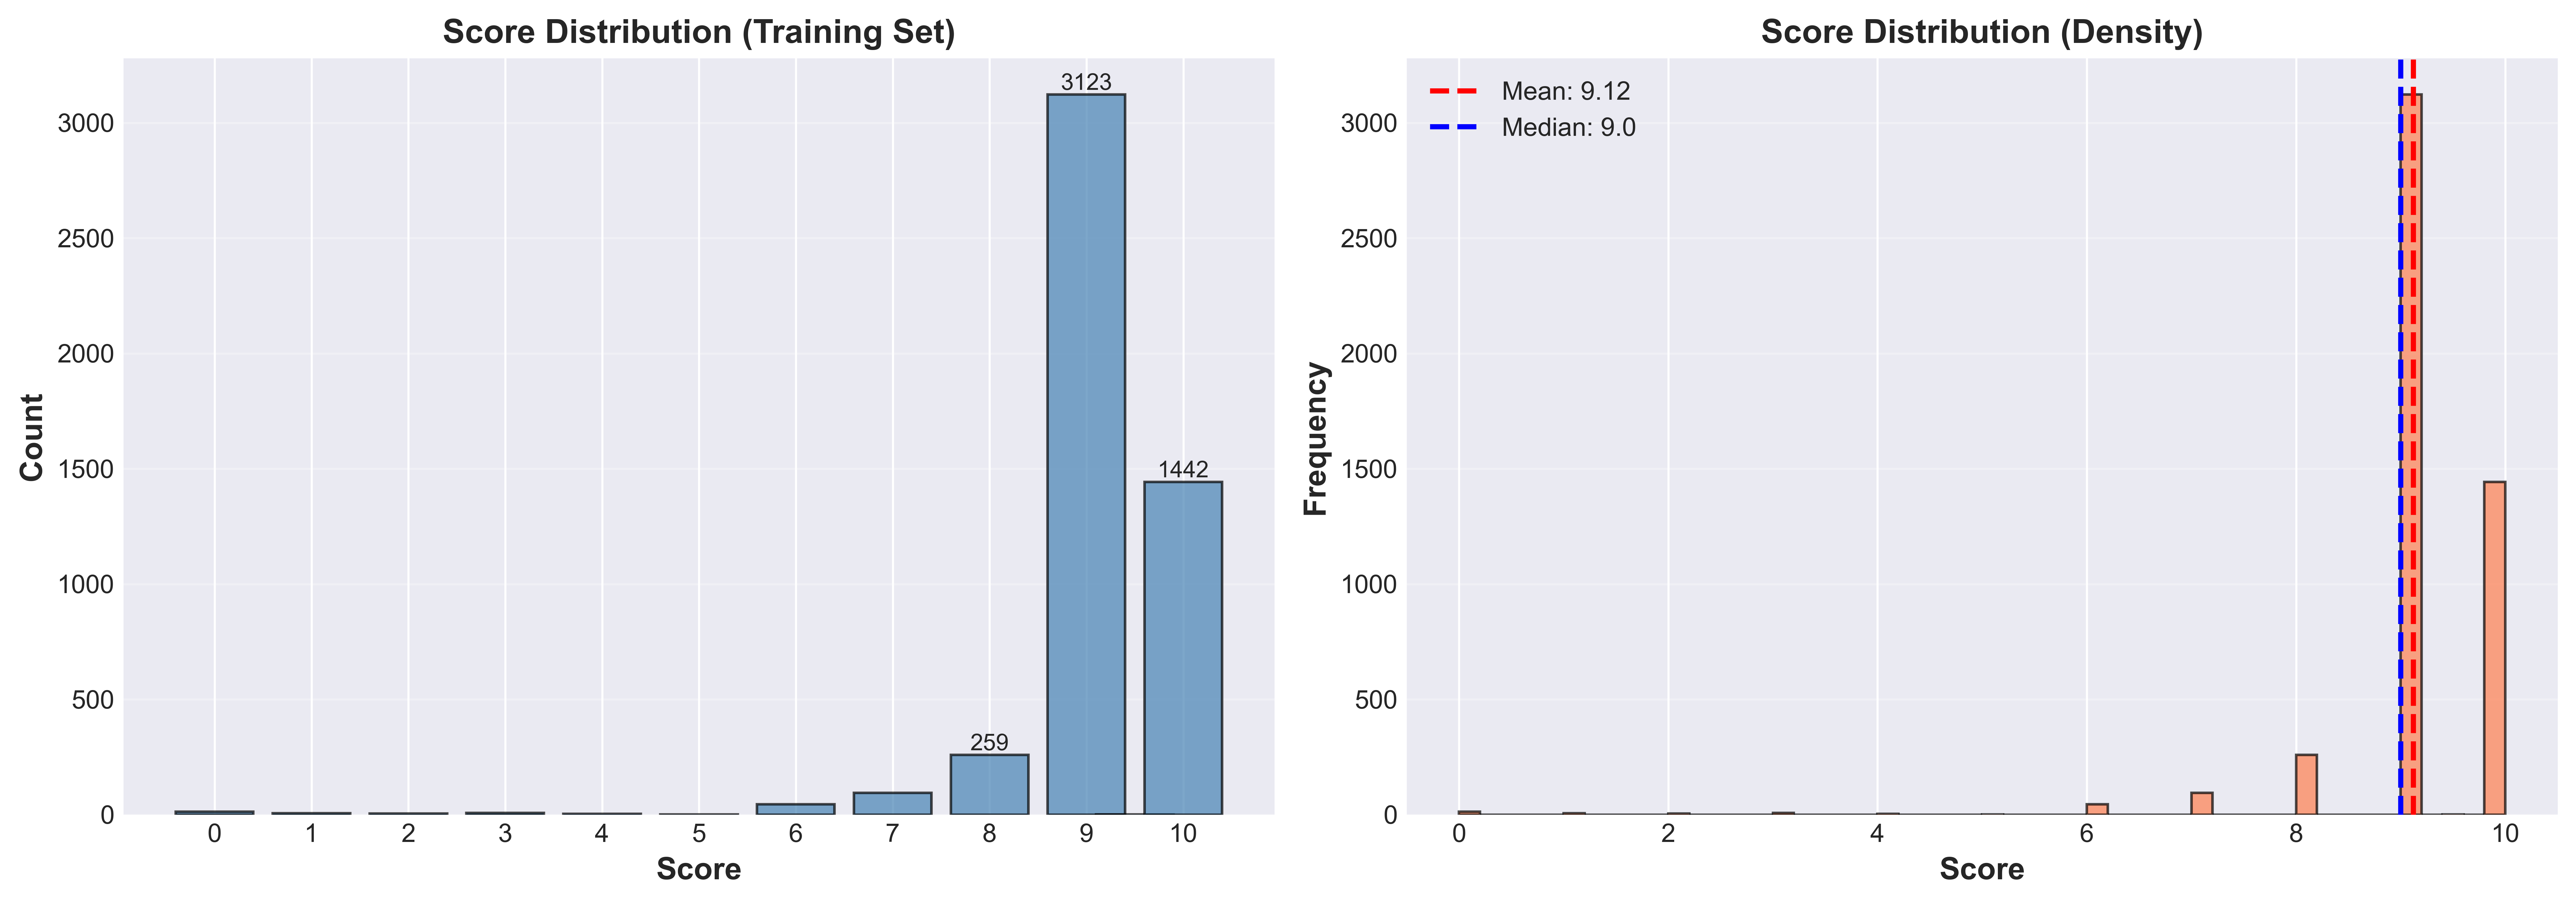
\includegraphics[width=0.85\textwidth]{plots/1_score_distribution.png}
  \caption{Training set score distribution. The distribution is heavily skewed toward high scores (majority 9--10).}
  \label{fig:score_dist_png}
\end{figure}

% --- 2. Metric sample count distribution
\begin{figure}[H]
  \centering
  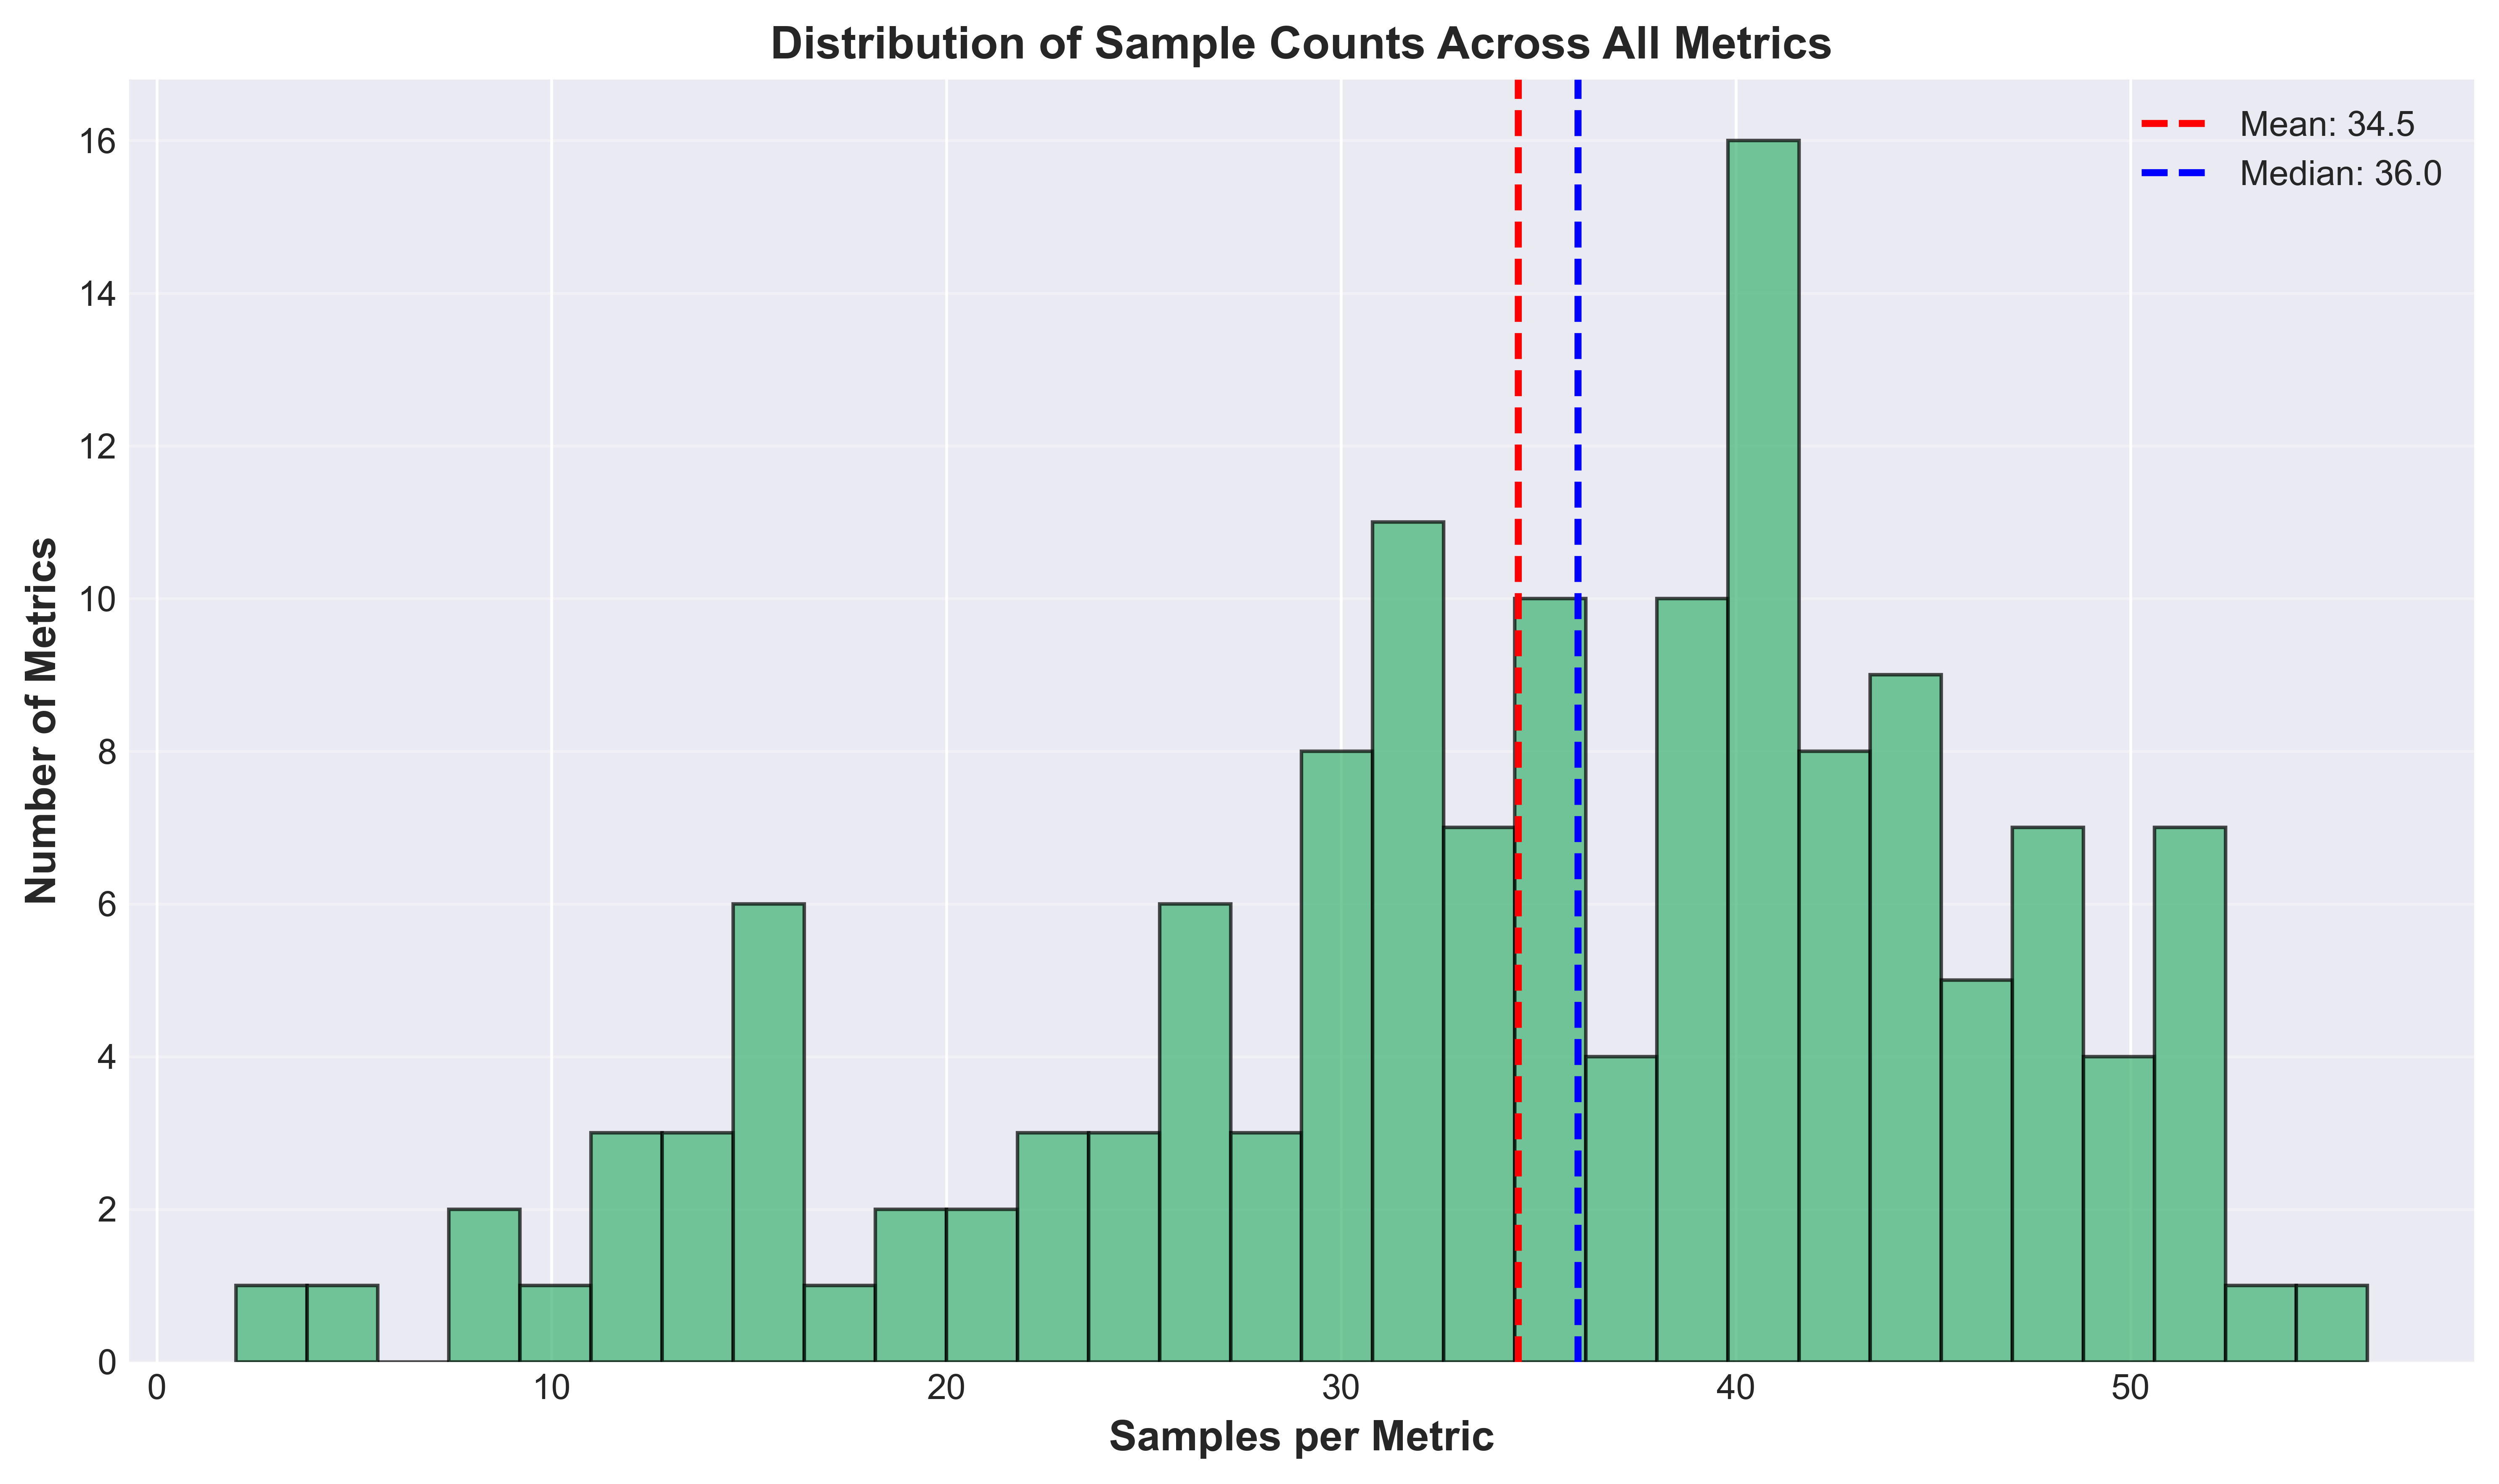
\includegraphics[width=0.85\textwidth]{plots/2_metric_sample_count_distribution.png}
  \caption{Per-metric sample counts. Metric support varies substantially (2--56 samples), with many metrics having low counts.}
  \label{fig:metric_counts_png}
\end{figure}

% --- 3. Text length distributions
\begin{figure}[H]
  \centering
  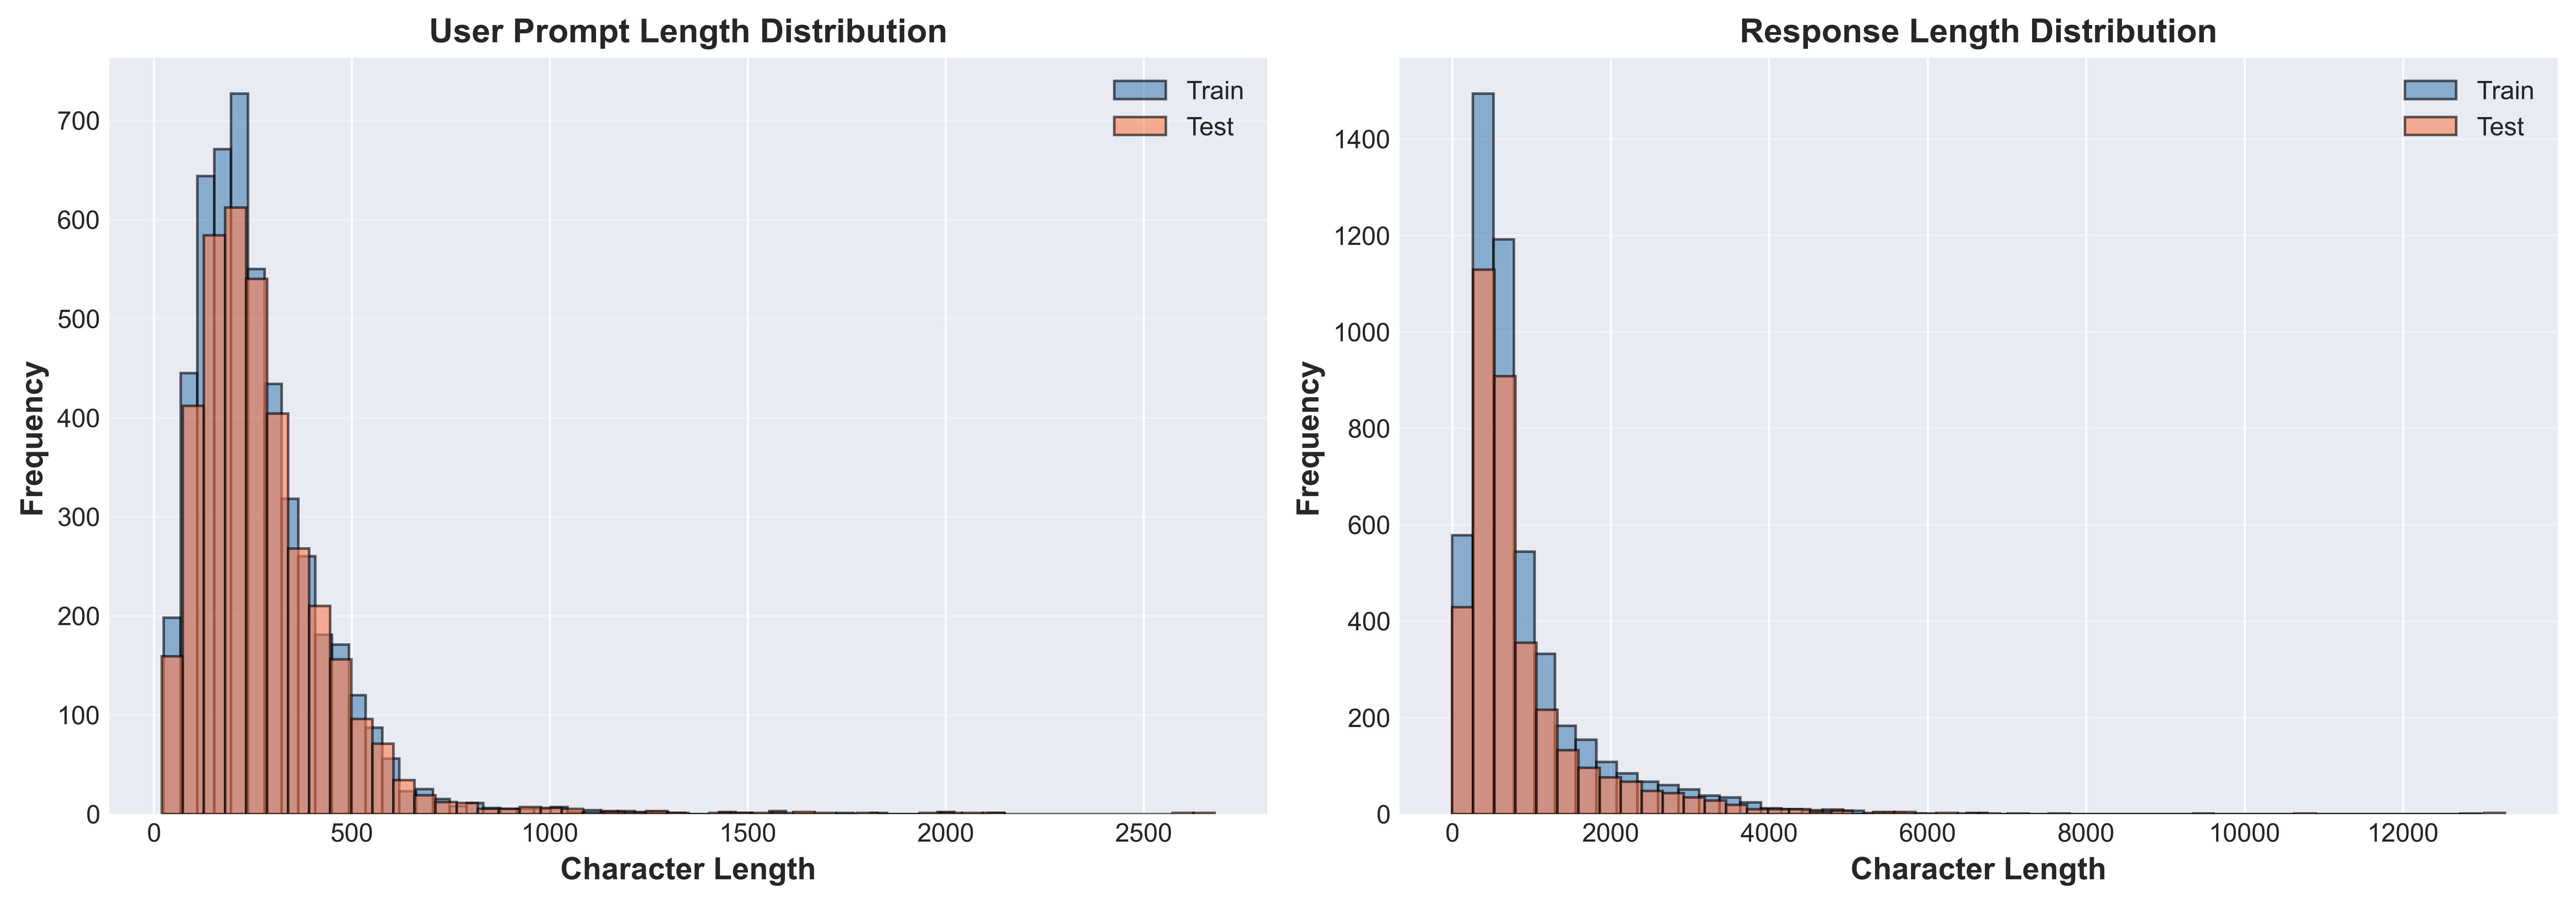
\includegraphics[width=0.85\textwidth]{plots/4_text_length_distributions.png}
  \caption{Character-length distributions for user prompts, system prompts, and responses. Response lengths show very wide variance (long tail up to ~13k characters).}
  \label{fig:lengths_png}
\end{figure}

% --- 4. Feature correlations (diagnostic)
\begin{figure}[H]
  \centering
  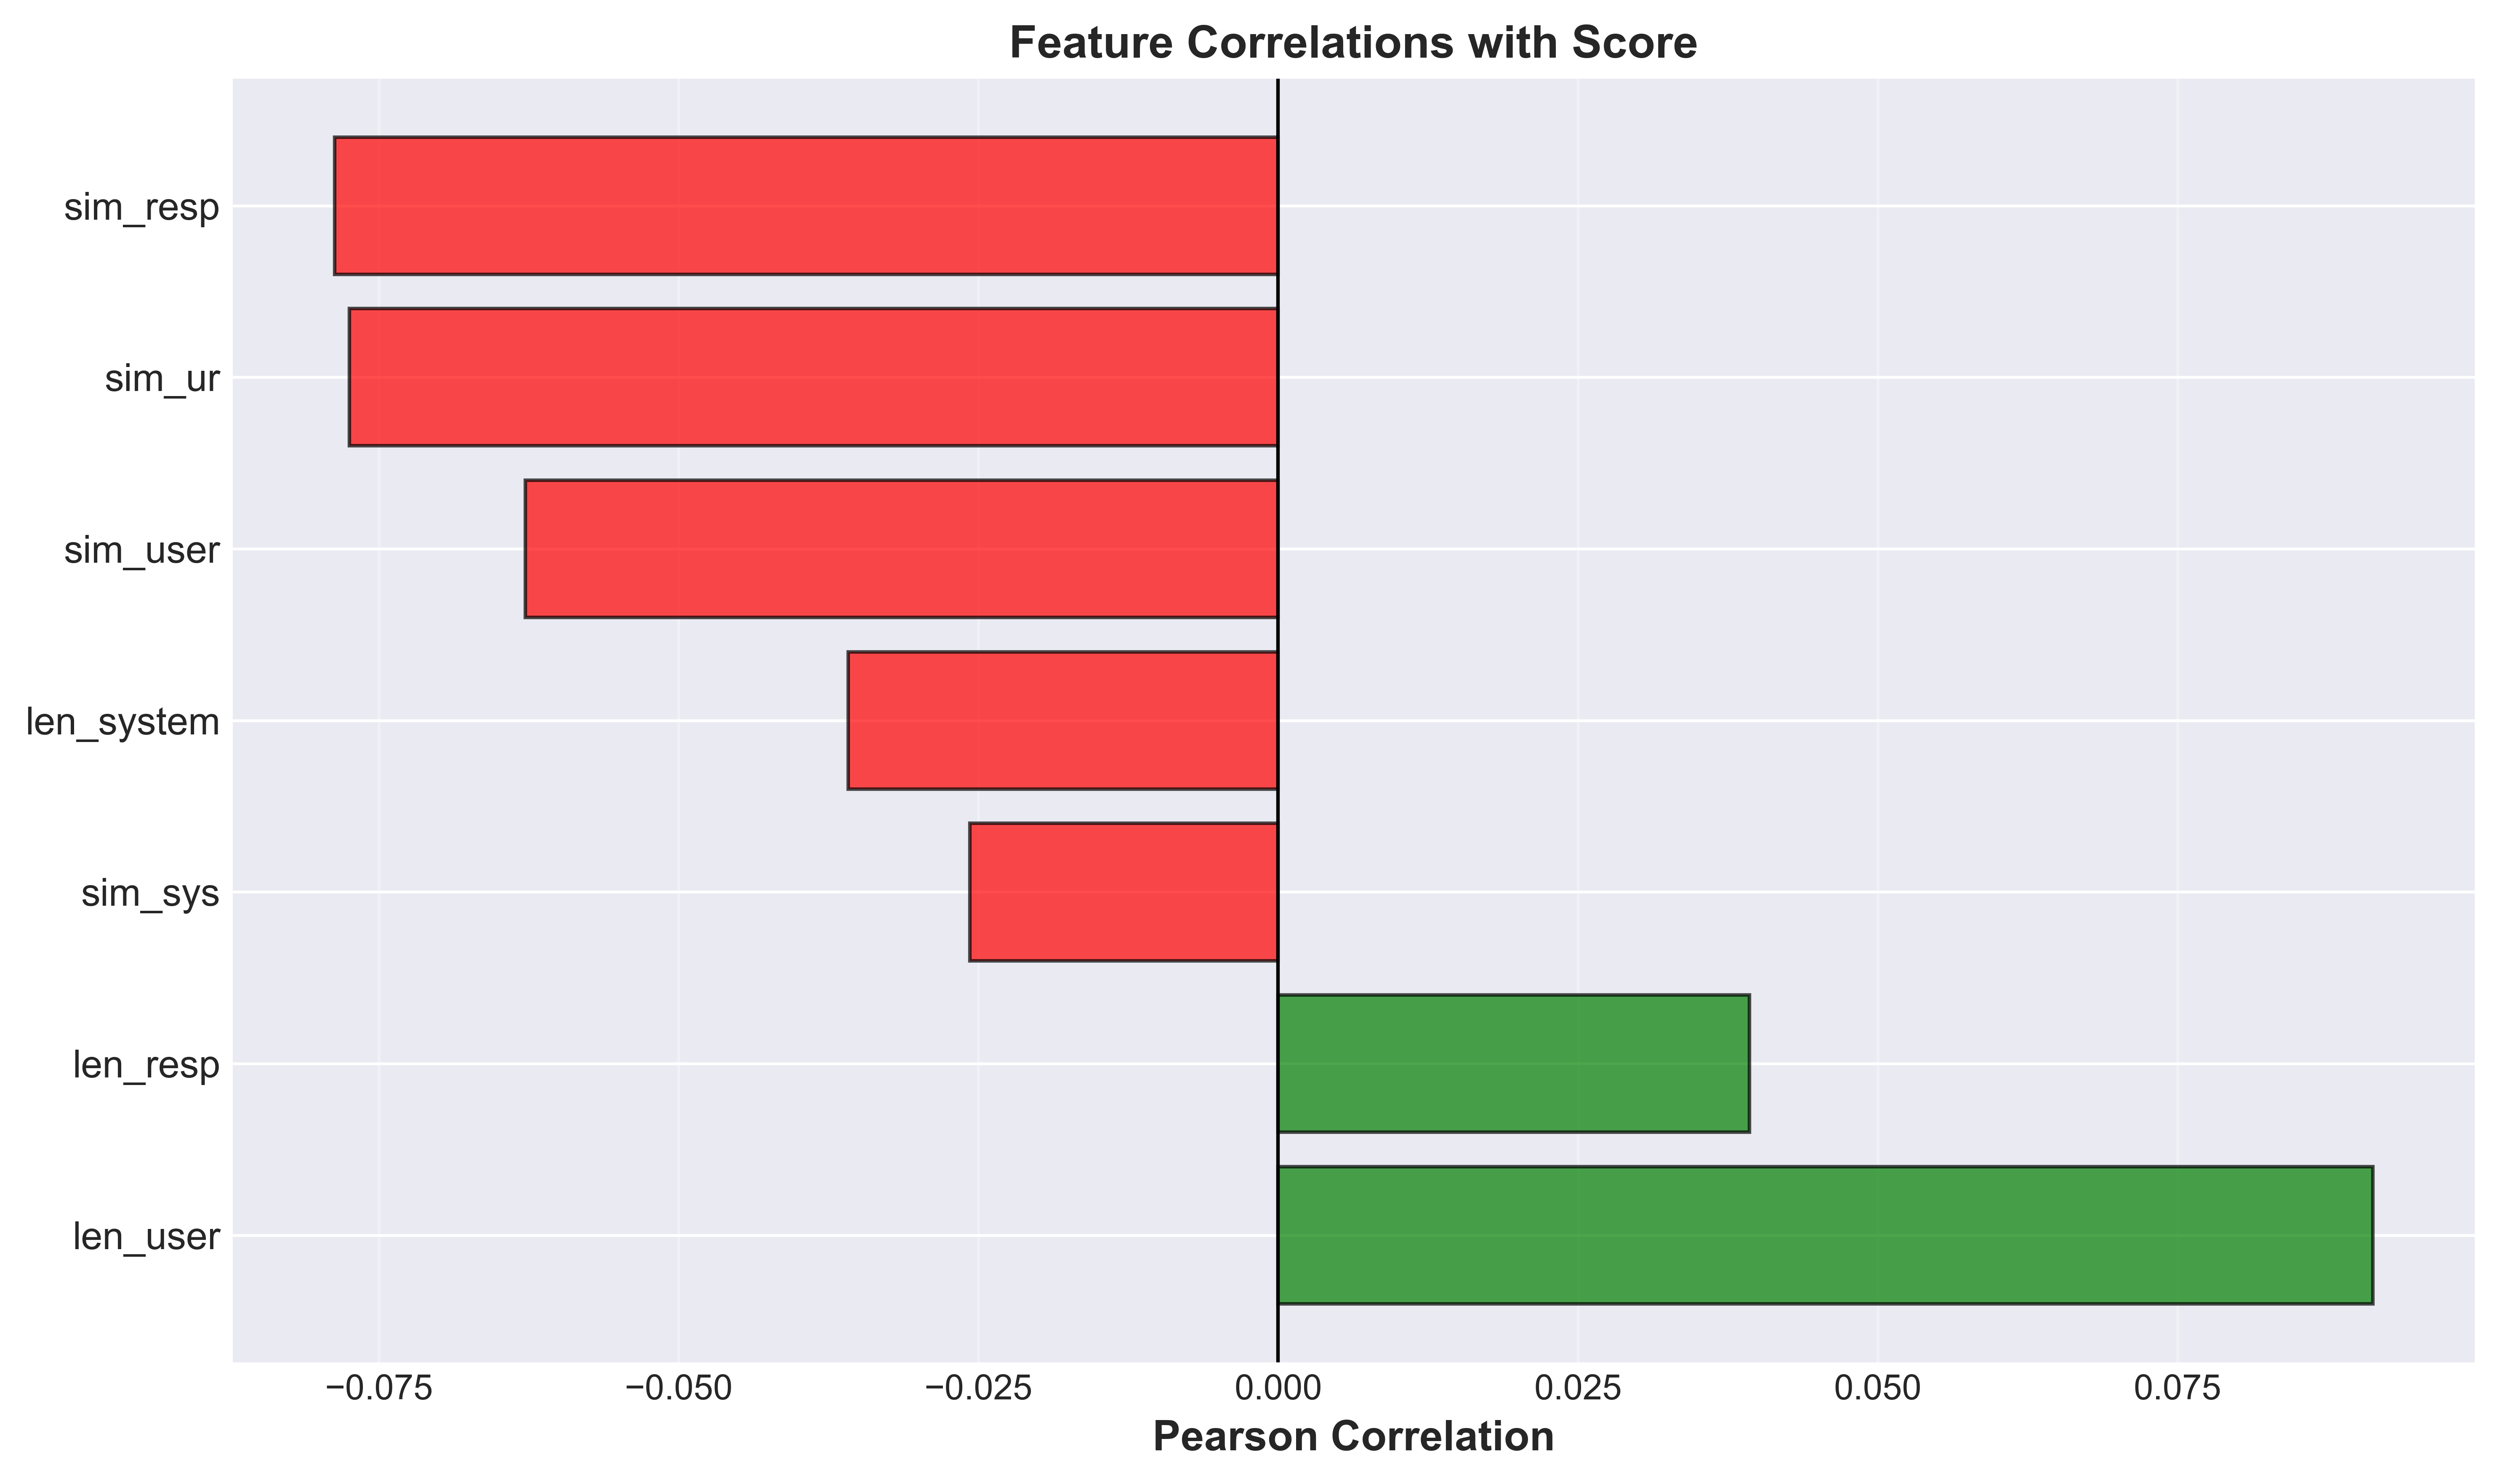
\includegraphics[width=0.75\textwidth]{plots/6_feature_correlations.png}
  \caption{Pearson correlations of simple features (lengths, cosine similarities) with score. Correlations are weak, indicating limited predictive power for simple heuristics.}
  \label{fig:correlations_png}
\end{figure}


\paragraph{Data quality and summary insights}
\begin{itemize}
    
    \item The dataset is extremely imbalanced (Fig.~\ref{fig:score_dist_png}), the mean and median of the scores for train set is 9.12 and 9.0 respectively. Any traditional approach will not be able to learn any low score distribution as the model only predicts higher values to always get lower error.

    \item The number of samples per Metric (145 in total) has a large variation from 2 to 56 (Fig.~\ref{fig:metric_counts_png}). The model might not be able to learn the distribution for metics with lower frequency. Some kind of per metric data augmentation is required.

    \item Text lengths, especially responses, show very large variance (Fig.~\ref{fig:lengths_png}). Some responses exceed 10{,}000 characters while others are nearly empty. We might need to use an embedding model that handles long-context variability without being dominated by outliers.

    \item System prompts are missing in roughly one-third of all samples. Since this distrubtion is similar for both train and test data, it might not play as big a role. 

    \item The dataset is multilingual and script-diverse. The majority of text is in Devanagari(Hindi) or Latin(English) scripts, but several other scripts also appear. This increases representational complexity.

    \item Cosine similarity features and simple length-based features show almost no correlation with the score (Fig.~\ref{fig:correlations_png}). This indicates that naive similarity-based/linear baselines cannot capture the semantic alignment needed for this task.

    \item All 145 metrics appear in both train and test splits, but the imbalance suggests that per-metric modelling, metric-aware sampling, or specialist models may be beneficial for handling rare or highly specific metrics.
    

\end{itemize}
\subsection{Baseline attempted}

\noindent I first implemented a LightGBM-based baseline to establish a performance floor and to tets a feature engineering pipeline. The approach consists of four main steps.

\begin{itemize}
    \item I computed cosine similarities between the precomputed metric embeddings (768 dimensions) and the Gemma-300M multilingual sentence embeddings for each text field: user prompt, response, system prompt, and their concatenation and used these as features. I also included simple features such as text lengths and per-metric shrinkage features. For each metric, I computed an out-of-fold (OOF) shrunk mean using GroupKFold to avoid data leakage. This gives a metric-specific prior that helps in cases where a metric has very few examples.  
    \item In addition, I created interaction features by taking the absolute difference and elementwise product between metric and text embeddings. I compressed these high-dimensional vectors using PCA to 128 dimensions to reduce the dimensionality and hopefullyimprove the model's performance.
    \item I trained a LightGBM regressor using 5-fold GroupKFold, grouping by \texttt{metric\_name}. This ensures that all samples from a metric appear together in the same fold, preventing metric-level leakage that would otherwise give overly optimistic validation results. The model uses standard regularization (L1/L2 penalties, feature and bagging fractions) and early stopping based on validation RMSE. 
    \item Raw LightGBM predictions were post-processed using isotonic regression. This method learns a monotonic mapping from the OOF predictions to the true labels. It corrects systematic miscalibration in the model and reduced OOF RMSE from 0.921 to 0.918. To handle metric-specific score biases, I fit a simple Ridge regression model that learns small per-metric offsets on top of the calibrated predictions. This step further improved OOF RMSE to 0.870. This shows that different metrics follow different score distributions, and adding metric-specific corrections is beneficial.
\end{itemize}


\subsection{Key observations, lessons and surprises}
The final baseline reached an OOF RMSE of 0.870, but its leaderboard score was 4.707, which is actually worse than the sample submission. I understood that the gap is mainly due to the heavy skew in the training data: the model learns to do well on the “easy” 9–10 region but generalises poorly elsewhere. The baseline was clearly overfitting to the dominant high-score patterns and made me realise the need for some kind of data augmentation or a mixed model approach.

% ======================================================================
\newpage
\section{Phase 1: Design Rationale and Experiments}

My design approach was heavily inspired by my observations and lessons form the pahse0.ipynb notebook. Few things that I had to keep in mind were:
\begin{itemize}
    \item The data is extremely imbalanced, so some form of data augmentation is imperative.
    \item Since we can't really impute scores of our own to the augmented data and also adding arbitrary scores might just make the problem worse, we need a loss function/method that does not require scores. 
    \item Seoarate the tasks into two parts: first learn to separate ``good'' and ``bad'' examples, then train specialist regressors for each group.
\end{itemize}

\paragraph{Data augmentation}
I use negative sampling for data augmentation. What it does is, for every good training example I have, it switches the metric name with a random metric name and uses that as a negative sample. This helps the model to learn the alignment between the text and the metric. Also it takes care of the problem where some metrics had lesser frequency. For each positive sample we can choose (K parameter) negative samples.

\paragraph{Using a Contrastive alignment model as a router.}
I pass every prompt--response embedding and the candidate metric embedding through a small MLP and treat the output as a compatibility score. Good pairs should score high, while metric-swapped (negative) pairs should score low. The training signal is a simple logistic contrastive loss with \(K\) negatives per anchor:
\begin{equation}
\label{eq:contrastive_loss}
\mathcal{L}_{\text{contrastive}} = -\frac{1}{N}\sum_{i=1}^{N}\left[ \log \sigma\!\left(s_i^{+}\right) + \frac{1}{K}\sum_{k=1}^{K}\log\left(1 - \sigma\!\left(s_{ik}^{-}\right)\right) \right]
\end{equation}
where \(s_i^{+}\) is the score for the true metric of sample \(i\) and \(s_{ik}^{-}\) are the scores for the \(K\) randomly swapped metrics. This loss does not need explicit labels for the negatives, so it fits perfectly with the augmentation strategy and keeps the router focused on pure alignment rather than the noisy score distribution.

\paragraph{Why specialist regressors are needed.}
I noticed that the contrastive model output is almost binary, the distribution of the scores centered around 0 and 9 like a donut gaussian. I decide to train two experts: a low-score head that over-samples failure cases and a high-score head that focuses on good scores. The low expert gets a weighted MSE so that rarer tail scores dominate its gradient:
\begin{equation}
\label{eq:low_weighted_mse}
\mathcal{L}_{\text{low}} = \frac{1}{|\mathcal{D}_{\text{low}}|}\sum_{(x,y)\in\mathcal{D}_{\text{low}}} \bigl[1 + \alpha\,\max(0, \tau - y)\bigr]\bigl(\hat{y}_{\text{low}}(x) - y\bigr)^2,
\end{equation}
where \(\tau=5\) is the routing threshold and \(\alpha\) controls how aggressively the extreme tail is emphasised.

\paragraph{Ranking loss for ordinal consistency.}
To keep predictions ordered correctly, every mini-batch forms positive pairs \((i,j)\) where \(y_i > y_j\). The ranking loss penalises the model if the higher-score sample fails to beat the lower-score one by at least a small margin \(m\):
\begin{equation}
\label{eq:ranking_loss}
\mathcal{L}_{\text{rank}} = \frac{1}{|\mathcal{P}|}\sum_{(i,j)\in\mathcal{P}} \max\bigl(0,\, m - (\hat{y}_i - \hat{y}_j)\bigr).
\end{equation}
Using this hinge-style loss stabilises training when the experts see similar content but different target scores, and it plugs directly into the joint objective in Eqn~\ref{eq:joint_loss}.

\paragraph{Joint training with contrastive loss.}
Initially I was using the contrastive model output to direct the data into one 
of two regressors, each trained on appropriate subsets of the data. But I found 
that the model was not able to learn the distribution of the scores very well. 
So I decided to train a joint model with the contrastive loss and the regression 
losses. This setup should encourage the router to learn a meaningful separation, 
and it should encourage the experts to learn better. The combined objective will 
let the alignment information and numeric prediction reinforce each other rather 
than competing. The global loss mixes the contrastive term (Eqn~\ref{eq:contrastive_loss}), the weighted low expert term (Eqn~\ref{eq:low_weighted_mse}), a standard high-score MSE, and the pairwise ranking loss (Eqn~\ref{eq:ranking_loss}):
\begin{equation}
\label{eq:joint_loss}
\mathcal{L}_{\text{joint}} = \lambda_c \mathcal{L}_{\text{contrastive}} + \lambda_{\ell} \mathcal{L}_{\text{low}} + \lambda_{h} \mathcal{L}_{\text{high}} + \lambda_{r} \mathcal{L}_{\text{rank}}.
\end{equation}
This single objective keeps the router grounded in alignment while giving it immediate feedback whenever a misrouted sample hurts the relevant expert.

\paragraph{Routing at inference.}
Inference is deterministic: I compare the contrastive score against the learnt threshold, send the sample to the matching expert, and return that expert's prediction. This mirrors the ``good vs bad'' decomposition observed in the data and keeps the decision rule transparent.

\paragraph{Rounding the predictions}
I rounded the predictions to the nearest integer using a custom heuristic. I ceil the scores $\leq 7$ and round the scores $> 7$. This is a simple heuristic to avoid systematic under-prediction. This gave much better results than simple rounding. My best submission was 0.2 points lower compared to the simple rounded submission.

\subsection{Different variants of the joint training approach}

\begin{itemize}
    \item \textbf{Pure contrastive router}: training only the metric/text router with Eqn~\ref{eq:contrastive_loss} and no regression heads. (This method gave me the best score on the leaderboard)
    \item \textbf{Score-aware contrastive}: treats samples with scores $\leq 6$ as additional negatives so the router becomes more sensitive to failing responses. (This method did not perform as well as the pure contrastive router)
    \item \textbf{Joint training (default)}: combining the router with low/high experts, weights the low expert using Eqn~\ref{eq:low_weighted_mse}, and optimising the joint loss in Eqn~\ref{eq:joint_loss}. 
    \item \textbf{Joint + ranking emphasis}: same as above but with a larger \(\lambda_r\) to enforce stronger ordinal constraints via Eqn~\ref{eq:ranking_loss}. This variant performed the best and is the one that I used for the final submission.
    \item \textbf{Joint without routing threshold}: ablates the hard routing decision by averaging the two experts' predictions using the router score as a soft gate; this performed worse and justified keeping the hard threshold.
\end{itemize}

\subsection{Results}
Against my expectations, the pure contrastive router performed the best and gave me the best score on the leaderboard. I had hoped that adding the regression heads and ranking loss would give me better performance as it made loical sense but I fell the lack of low score data was the reason for the poor performance. If I had more time, I would try more hyperparameter tuning and data augmentation techniques to improve the performance. The number of epochs in particular and the weights of the different loss components. The lower score regression model might have done a better job with less epochs so that it dosent overfit on the limited data available. Below is a plot that shows the distribution of the test pred scores for the current exp file in phase1.ipynb against some previous good ones.
\begin{figure}[H]
  \centering
  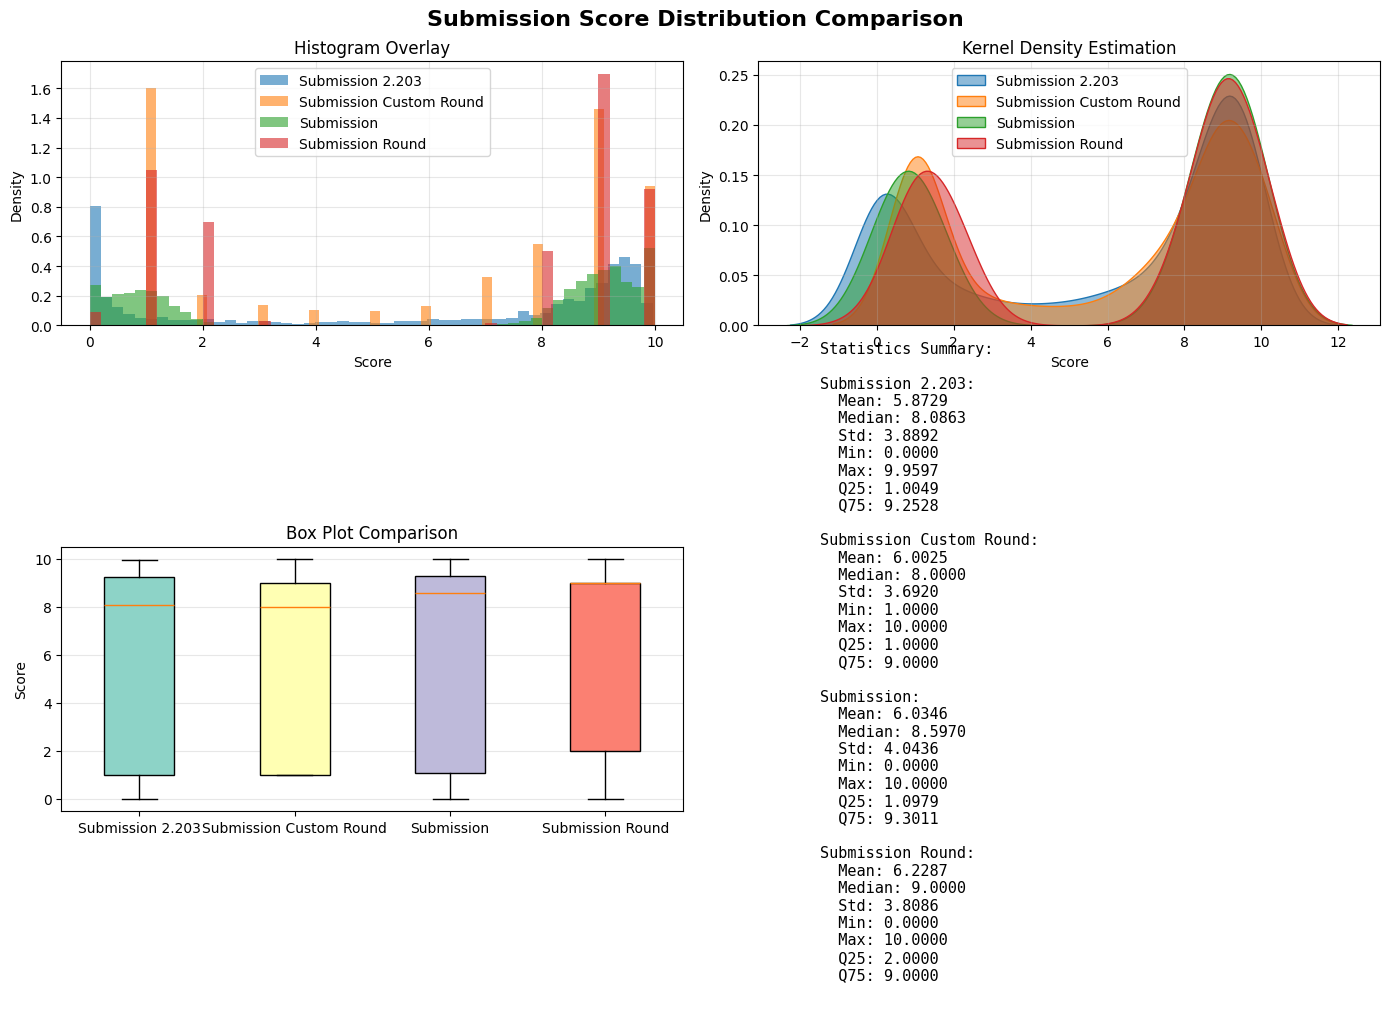
\includegraphics[width=1.0\textwidth]{plots/final_dist.png}
  \caption{Distribution of the test pred scores for the current exp file in phase1.ipynb against some previous good ones. Submission Custom round is the best submission.}
  \label{fig:submission_distributions_png}
\end{figure}

\newpage
\section{Best Submission}
The code and instructions for reproducing my Best Submission are available on GitHub at \url{https://github.com/mnm-21/da5401_project}.
\label{sec:best}
\subsection{Model components}
\begin{itemize}
  \item \textbf{Embedding stack}: \texttt{google/embeddinggemma-300m} encodes every (system, user, response) triple plus the 145 metric descriptions into 768-d vectors. The resulting arrays live in \texttt{saved\_embeddings/*.npy} for deterministic reuse.
  \item \textbf{MetricModel router}: a 2-layer MLP \((1536 \rightarrow 512 \rightarrow 1)\) with ReLU + Dropout~0.1 that concatenates text and metric embeddings and produces a logit. Training uses the logistic contrastive loss in Eqn~\ref{eq:contrastive_loss} with \(K=2\) negatives per anchor.
  \item \textbf{10-fold stratified CV}: scores are discretised with \texttt{KBinsDiscretizer} (10 bins) before running \texttt{StratifiedKFold}. Each fold trains for 20 epochs; fold~9 (MSE \(=3.459\)) becomes the frozen checkpoint for inference.
  \item \textbf{Sigmoid-to-score mapping}: inference applies \(\hat{s}=10\cdot\sigma(z)\) to convert logits into the 0--10 range. This is the only scaling; no external regressors or calibration layers were needed for the winning run.
  \item \textbf{Rounding heuristic}: raw predictions go to \texttt{submission.csv}, while the leaderboard file \texttt{submission\_custom\_round.csv} ceilings scores \(\leq 7\) and rounds the rest, preventing systematic underestimation of weak answers.
\end{itemize}

\subsection{Exact training \& inference recipe}
\begin{enumerate}
  \item \textbf{Prepare text inputs}: format each row as \texttt{title: none | text: system [SEP] user [SEP] response} and cache Gemma embeddings via \texttt{encode\_texts\_if\_needed}.
  \item \textbf{Load metric bank}: embed all metric names once (\texttt{metric\_name\_embeddings.npy}) and build a lookup map.
  \item \textbf{Contrastive CV}: for each of the 10 folds, instantiate \texttt{MetricModel}, train for 20 epochs with \texttt{train\_contrastive} (batch size 128, \(K=2\) negatives), and evaluate MSE on the held-out fold.
  \item \textbf{Checkpoint selection}: pick the fold with the lowest validation MSE (fold 9) and reload its \texttt{state\_dict}.
  \item \textbf{Test inference}: run \texttt{predict\_scores} on all test embeddings, multiply sigmoid outputs by 10, and save \texttt{submission.csv}.
  \item \textbf{Rounded submission}: apply the heuristic \texttt{score = ceil(score)} if \texttt{score <= 7} else \texttt{round(score)} to get \texttt{submission\_custom\_round.csv}, the file uploaded to Kaggle.
\end{enumerate}

\newpage
\section{Conclusion}
\label{sec:conclusion}
The final contrastive-only router, paired with the lightweight rounding rule, ended up giving the best leaderboard score. The takeaways I have from this project are: (i) clean alignment signals matter more than complex downstream regressors when data is scarce, and (ii) the low-score still needs targeted augmentation before specialist (regression) heads can help. If I continue the project, I would focus on getting more low-score examples, experimenting with softer routing (temperature-scaled logits or distillation), and tuning the joint loss weights with proper Bayesian search instead of hand-picked values. Using a finer classification might also benefit where we recursively classify into good and bad and finally combine our classes into 10 distinct ones. I didn't have time to implement this but it would be a good idea to try.

\appendix
\section{Supplementary plots}
\label{app:plots}
All figures generated during exploration and submission analysis are available in the \texttt{plots/} folder (committed to git). The complete list is organized below:

\paragraph{Score and metric distributions}
\begin{itemize}[leftmargin=1.5em]
  \item \texttt{1\_score\_distribution.png}: train vs test score histograms showing the extreme skew toward 9--10.
  \item \texttt{2\_metric\_sample\_count\_distribution.png}: distribution of sample counts per metric (highly imbalanced).
  \item \texttt{3\_metric\_mean\_score\_distribution.png}: distribution of mean scores across all 145 metrics.
  \item \texttt{7\_metric\_variance\_distribution.png}: per-metric score variance distribution.
  \item \texttt{per\_metric\_1\_sample\_count\_dist.png}: detailed per-metric sample count analysis.
  \item \texttt{per\_metric\_2\_mean\_score\_dist.png}: per-metric mean score breakdown.
  \item \texttt{per\_metric\_3\_scatter.png}: scatter plots showing score distributions for individual metrics.
  \item \texttt{per\_metric\_4\_all\_metrics\_by\_count.png}: comprehensive view of all metrics sorted by sample count.
  \item \texttt{per\_metric\_analysis.png}: combined per-metric diagnostic dashboard.
\end{itemize}

\paragraph{Text length and script analysis}
\begin{itemize}[leftmargin=1.5em]
  \item \texttt{4\_text\_length\_distributions.png}: distributions of user prompt and response lengths.
  \item \texttt{9\_score\_vs\_length.png}: scatter plot showing score vs response length relationship.
  \item \texttt{text\_script\_1\_length\_boxplot.png}: text length distributions broken down by script type (boxplots).
  \item \texttt{text\_script\_2\_script\_pie.png}: pie chart showing script distribution in the dataset.
  \item \texttt{text\_script\_3\_cumulative\_length.png}: cumulative length distributions by script.
  \item \texttt{text\_script\_4\_all\_transitions.png}: transition matrix showing user-script → response-script patterns.
  \item \texttt{text\_length\_script\_analysis.png}: comprehensive multi-panel analysis of text lengths and scripts.
\end{itemize}

\paragraph{System prompts and feature correlations}
\begin{itemize}[leftmargin=1.5em]
  \item \texttt{8\_system\_prompt\_presence.png}: missingness vs presence counts for system prompts, annotated with percentages.
  \item \texttt{5\_script\_combinations\_all.png}: full user-script → response-script transition heatmap showing all script pairs.
  \item \texttt{6\_feature\_correlations.png}: correlation analysis between engineered features.
  \item \texttt{correlation\_heatmap.png}: Pearson correlation heatmap across all features including Gemma similarity scores.
\end{itemize}

\paragraph{Summary and submission analysis}
\begin{itemize}[leftmargin=1.5em]
  \item \texttt{data\_exploration\_summary.png}: comprehensive summary dashboard combining key insights from all analyses.
  \item \texttt{final\_dist.png}: comparison of submission score distributions (best round vs earlier baselines); this is the figure embedded in Figure~\ref{fig:submission_distributions_png}.
\end{itemize}

\section{Core PyTorch blocks in Best Submission}

\begin{lstlisting}[language=Python]
class MetricModel(nn.Module):
    def __init__(self, text_dim=768, metric_dim=768,
                 hidden_dim=512, dropout=0.1):
        super().__init__()
        self.net = nn.Sequential(
            nn.Linear(text_dim + metric_dim, hidden_dim),
            nn.ReLU(),
            nn.Dropout(dropout),
            nn.Linear(hidden_dim, 1),
        )

    def forward(self, text_emb, metric_emb):
        combo = torch.cat([text_emb, metric_emb], dim=-1)
        return self.net(combo)


def contrastive_loss(pos_scores, neg_scores):
    pos_term = -torch.log(torch.sigmoid(pos_scores) + 1e-8).mean()
    if neg_scores.dim() == 2:  # K negatives per anchor
        neg_term = -torch.log(1 - torch.sigmoid(neg_scores) + 1e-8).mean()
    else:
        neg_term = -torch.log(1 - torch.sigmoid(neg_scores) + 1e-8).mean()
    return pos_term + neg_term
\end{lstlisting}

\begin{lstlisting}[language=Python]
import math
import pandas as pd

def final_rounding(score: float) -> int:
    return math.ceil(score) if score <= 7 else round(score)

sub = pd.read_csv("submission.csv")
sub["score"] = sub["score"].apply(final_rounding)
sub.to_csv("submission_custom_round.csv", index=False)
\end{lstlisting}

\end{document}